\section{Your project idea/description}

In this section, first, we redefine the problem in great detail. Then, describe your solutions. Try to use as many illustrations, such as pictures, graphs, and pseudo-codes, as you see fit. Here are some examples of including pictures, graphs, and pseudo-code in latex. 

%%%%%%%%%%%%%%%%%%%%%%%%%%%%%%%%%%%%%%%%%%%%%%%%%%%%%%%%%%%%%%%%%%%
%
% Commands to include a figure:
%
%%%%%%%%%%%%%%%%%%%%%%%%%%%%%%%%%%%%%%%%%%%%%%%%%%%%%%%%%%%%%%%%%%%
Figure~\ref{fig:fig1} shows how to include a picture in a Latex document. 
\begin{figure}[!ht]
 \centering

\includegraphics[width=3in]{figures/sample_1.jpg}
\caption{\label{fig:fig1}This is my great security design.}
\end{figure}

%%%%%%%%%%%%%%%%%%%%%%%%%%%%%%%%%%%%%%%%%%%%%%%%%%%%%%%%%%%%%%%%%%%
%
% The following pseudo code is copied from 
% http://users.sdsc.edu/~ssmallen/latex/pseudocode.html
%
%%%%%%%%%%%%%%%%%%%%%%%%%%%%%%%%%%%%%%%%%%%%%%%%%%%%%%%%%%%%%%%%%%%
Figure~\ref{fig:fig2} is a sample pseudo code copied from this site \cite{pseudocode}. 

\begin{figure}[!ht]
 \centering
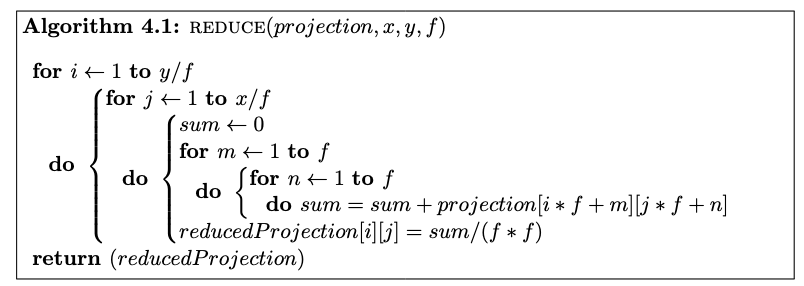
\includegraphics[width=3in]{figures/algorithm.png}

  \caption{\label{fig:fig2}This is my great pseudocode}
  
  \end{figure}





%%%%%%%%%%%%%%%%%%%%%%%%%%%%%%%%%%%%%%%%%%%%%%%%%%%%%%%%%%%%%%%%%%%
%
% Latex float chart example
% Copied from http://www.texample.net/tikz/examples/simple-flow-chart/
%
%%%%%%%%%%%%%%%%%%%%%%%%%%%%%%%%%%%%%%%%%%%%%%%%%%%%%%%%%%%%%%%%%%%

Figure~\ref{fig:fig3} is a sample float chart copy from this website \cite{floatchart}
   
  \begin{figure}[!ht]
 \centering
 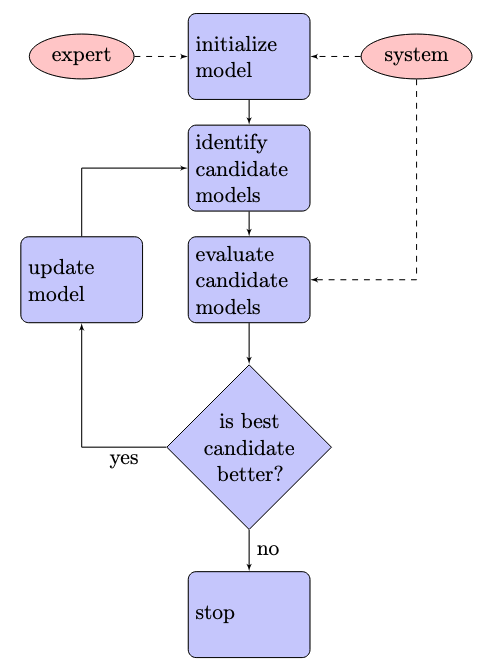
\includegraphics[width=3in]{figures/flowchart.png}

  \caption{\label{fig:fig3}This is my great float chart}
  
  \end{figure}


%%%%%%%%%%%%%%%%%%%%%%%%%%%%%%%%%%%%%%%%%%%%%%%%%%%%%%%%%%%%%%%%%%%

\subsection{Mathematics}

If your project idea needs mathematics to formulate your methods, \LaTeX{} is great at typesetting mathematics. Let $X_1, X_2, \ldots, X_n$ be a sequence of independent and identically distributed random variables with $\text{E}[X_i] = \mu$ and $\text{Var}[X_i] = \sigma^2 < \infty$, and let
$$S_n = \frac{X_1 + X_2 + \cdots + X_n}{n}
      = \frac{1}{n}\sum_{i}^{n} X_i$$
denote their mean. Then as $n$ approaches infinity, the random variables $\sqrt{n}(S_n - \mu)$ converge in distribution to a normal $\mathcal{N}(0, \sigma^2)$.
